\section{Three-way tables}\label{sec:mosaic-threeway}

The mosaic display can be extended to three- and higher-way tables.
The relative frequencies of a third variable are used to subdivide
each two-way cell, and so on, recursively.

Imagine that each
cell of the two-way table for Hair and Eye color is further
classified by one or more additional variables---sex and level of
education, for example.  Then each rectangle can be subdivided
horizontally to show the proportion of males and females in that
cell, and each of those horizontal portions can be subdivided
vertically to show the proportions of people at each educational
level in the hair-eye-sex group.

\figref{fig:mosaic35} shows the mosaic for the three-way table, with Hair and Eye color
groups divided according to the proportions of Males and Females:
We see that there is no systematic association between sex
and the combinations of Hair and Eye color---except among
blue-eyed blonds, where there are an overabundance of females.

\begin{figure}[!htb]
  \centering
  \includegraphics[scale=.6]{ch4/fig/mosaic35}
  \caption[Three-way mosaic, joint independence]{Three-way mosaic display for hair color, eye
color, and sex.
The categories of sex are crossed with those of
hair color, but only the first occurrence is labeled.
Residuals from
the model of joint independence, \([HE]\,  [S]\) are shown by
shading.
\(G^2\) = 19.86 on 15 df.
The only lack of fit is
an overabundance of females among blue-eyed blonds.}
\label{fig:mosaic35}
\end{figure}

\subsection{Fitting models}\label{sec:mosaic-fitting}
When three or more variables are
represented in the mosaic, we can fit several different models of
``independence'' and display the residuals from each model.  We treat
these models as null or baseline models, which may not fit the data
particularly well.  The deviations of observed frequencies from
expected ones, displayed by shading, will often suggest terms to be added
to an explanatory model that achieves a better fit.

For a three-way table, with variables $A$, $B$ and $C$, some of the hypothesized models which can be fit are
described below and summarized in \tabref{tab:hyp3way}.
Here I use $[\,]$ notation to list the \emph{high-order terms} in
a hierarchical \loglin{} model; these correspond to the margins
of the table which are fitted exactly.  The notation \LLM{AB,AC},
for example, is shorthand for the model
\begin{equation*}
  \log \,  m_{ijk}  =
  \mu  +  \lambda_i^A
  +  \lambda_j^B
  +  \lambda_k^C
  +  \lambda_{ij}^{AB}
  +  \lambda_{ik}^{AC}
  \comma
\end{equation*}
as described in \secref{sec:loglin-counts}, and reproduces the
$\{AB\}$ and $\{AC\}$ marginal subtables.
Here, $A \perp B$ is
read, ``$A$ is independent of $B$.''  \tabref{tab:hyp3way} also
depicts the relations among variables as an
association graph, where associated variables are connected by an edge.

Each model fits certain table margins exactly, as shown in the table;
other associations present in the data will appear in the pattern of
residuals.
\begin{description}
\item[$H_1$: Complete independence.]  The model of complete (mutual) independence, symbolized $A \perp B \perp C$,
       asserts that all joint probabilities are products of the
       one-way marginal probabilities:
\begin{equation*}
 \pi_{ijk} = \pi_{i++} \: \pi_{+j+} \: \pi_{++k}
 \comma
\end{equation*}
for all \(i , j , k\) in a
       three-way table.  This corresponds to the log-linear model
       \LLM{A,B,C}.  Fitting this model puts all higher
       terms, and hence all association among the variables, into the
       residuals.
\item[$H_2$: Joint independence.]  Another possibility is to fit the model in
       which variable \(C\) is jointly independent of variables \(A\)
       and \(B\), ($A , B \perp C $), where
\begin{equation*}
 \pi_{ijk}  =  \pi_{ij+} \:  \pi_{++k} \period
\end{equation*}
This corresponds to the log-linear model \LLM{AB,C}.
Residuals from this model show the extent to which
variable \(C\) is related to the combinations of variables
\(A\) and \(B\) but they do not show any association between
\(A\) and \(B\), since that association is fitted exactly.
For this model, variable $C$ is also independent of $A$ and
$B$ in the marginal $\{AC\}$ table (collapsing over $B$) and
in the marginal $\{BC\}$.

\item[$H_3$: Conditional independence.] Two variables, say $A$ and $B$ are conditionally independent
given the third ($C$) if $A$ and $B$ are independent when we
control for $C$, symbolized as $A \perp B \given C$.
This means that conditional probabilities, $\pi_{ij|k}$ obey
\begin{equation*}
 \pi_{ij|k}  =  \pi_{i+|k} \:  \pi_{+j|k} \comma
\end{equation*}
where
$\pi_{ij|k} = \pi_{ijk} / \pi_{ij+}$,
$\pi_{i+|k} = \pi_{i+k} / \pi_{i++}$, and
$\pi_{+j|k} = \pi_{+jk} / \pi_{+j+}$.
The corresponding \loglin{} models is denoted \LLM{AC,BC}.
When this model is fit, the mosaic display shows the conditional
associations between variables $A$ and $B$, controlling for $C$,
but does not show the associations between $A$ and $C$, or
$B$ and $C$.

\item[$H_4$: No three-way interaction.]  For this model, no pair is
marginally or
conditionally independent, so there is \emph{no} independence interpretation.
Nor is there a closed-form expression for the cell probabilities.
However, the association between any two
variables is the same at each level of the third variable.
The corresponding \loglin{} model formula is \LLM{AB,AC,BC},
indicating that all two-way margins are fit exactly and so are not
shown in the mosaic residuals.
\end{description}
\begin{comment}
\newcommand{\tridot}[1]{%
	\begin{pspicture}(-.01, -.01)(1.1,1.1)%
	\psset{xunit=.85cm,yunit=.85cm}%
	\color{black}%
	\rput(0,0){\circlenode{A}{\textsf{A}}}%
	\rput(1.0,0){\circlenode{B}{\textsf{B}}}%
	\rput(.5,.866){\circlenode{C}{\textsf{C}}}%
	#1%
	\end{pspicture}%
	\rule{0in}{1.2cm}
%	}
}
\end{comment}

\newcommand{\tridot}[1]{%
\begin{tikzpicture}[x=0.85cm, y=0.85cm]
  \node(A)[draw, circle, fill=yellow!30] at (0,0) {\textbf{\textsf{A}}};
  \node(B)[draw, circle, fill=yellow!30] at (1,0) {\textbf{\textsf{B}}};
  \node(C)[draw, circle, fill=yellow!30] at (.5,.866) {\textbf{\textsf{C}}};
  #1%
%  \path (A) edge (B);
%  \path (B) edge (C);
%  \draw (0,0) circle 
\end{tikzpicture}
}

\begin{table}[htb]
\caption[Hypotheses for a three-way table]{Fitted margins, model symbols and interpretations for some hypotheses for a three-way table}\label{tab:hyp3way}
\begin{center}
  \begin{tabular}{|clllc|} \hline
             & Fitted  & Model &  Independence  & Association  \\
  Hypothesis & margins & symbol & Interpretation & graph \\
   \hline 
  $H_1$ & $n_{i++}, n_{+j+}, n_{++k}$ & [A][B][C] & $A \perp B \perp C $ & 
  \tridot{} \\[3ex] 
  $H_2$ & $n_{ij+}, n_{++k}$ & [AB][C] & $(A , B )\perp C $ & 
  \tridot{\path (A) edge (B);} \\[3ex]
%
  $H_3$ & $n_{i+k}, n_{+jk}$ & [AC][BC] & $A \perp B \: |\: C$ & 
  \tridot{\path (A) edge (C); \path (B) edge (C);} \\[3ex]
  $H_4$ & $n_{ij+}, n_{i+k}, n_{+jk}$ & [AB][AC][BC] & \texttt{NA} & 
  \tridot{\path (A) edge (B); \path (B) edge (C); \path (A) edge (C);} \\[3ex]
%
  \hline
  \end{tabular}
 \end{center}
\end{table}



For example, with the data from \tabref{tab:hairdat} broken down
by sex, fitting the joint-independence model [HairEye][Sex] allows us to see the extent
to which the joint distribution of hair color and eye color is
associated with sex.  For this model, the likelihood-ratio \(G^2\) is
19.86 on 15 \(df\) (\(p  =  .178\)), indicating an acceptable overall fit.
The three-way mosaic for this model was shown in \figref{fig:mosaic35}.
Any other model fit to this table will have the same size tiles in the mosaic
since the areas depend on the observed frequencies;  the residuals,
and hence the shading of the tiles will differ.
Thus, fitting a conditional independence model, [HairSex][EyeSex]
would test whether, given sex, hair color and eye color are independent
(probably not a meaningful hypothesis, here).
This model fits very poorly ($G^2 (18) = 156.68$).
The mosaic display, shown in \figref{fig:mosaic36}, has a pattern
similar to that in the two-way display, \figref{fig:mosaic34}.

\begin{figure}[!htb]
  \centering
  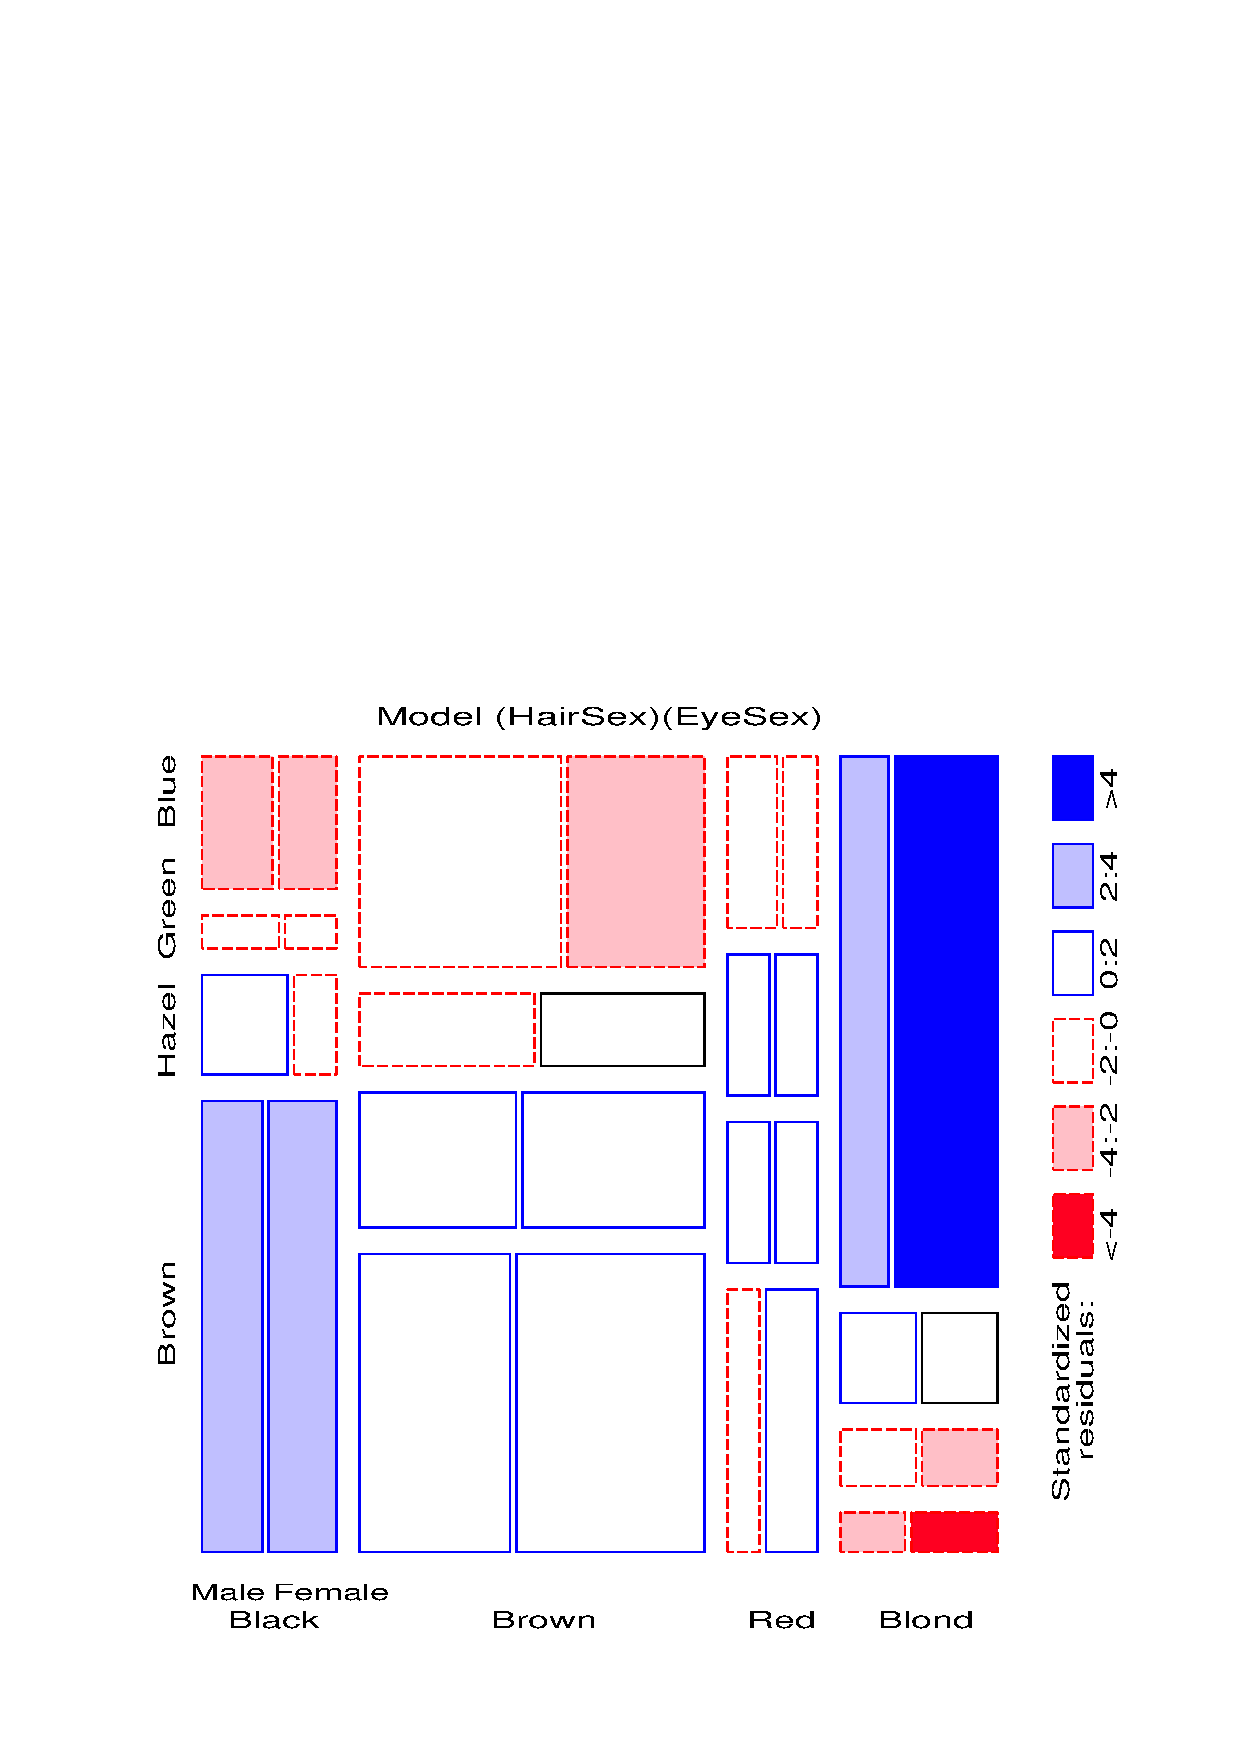
\includegraphics[scale=.6]{ch4/fig/mosaic36}
  \caption[Three-way mosaic, conditional independence]{Mosaic display for hair color, eye
color, and sex.  This display shows residuals from the model of
conditional independence, \([HS] \,  [ES] \), \(G^2\) = 156.68 on 18 df.}
  \label{fig:mosaic36}
\end{figure}

\subsubsection{Sequential plots and models}\label{sec:mosaic-seq}

The mosaic display is constructed in stages, with the variables
listed in a given order.
At each stage, the procedure
fits a (sub)model to the marginal subtable defined by summing over all
variables not yet entered.  For example for a three-way table,
$\{ABC\}$, the marginal subtables $\{A\}$ and $\{AB\}$ are calculated
in the process of constructing the three-way mosaic.
The $\{A\}$ marginal table can be fit to a model where the categories
of variable A are equiprobable (or some other discrete distribution);
the independence model can be fit to the $\{AB\}$ subtable, and so forth.

The series of plots can give greater insight into the relationships
among all the variables than a single plot alone.
Moreover, the series of mosaic plots fitting submodels of
joint independence to
the marginal subtables have the special property that they can be viewed as partitioning the hypothesis
of mutual independence in the full table.

For example, for the hair-eye data, the mosaic displays for the
\llmterm{Hair} \llmterm{Eye} marginal table (\figref{fig:mosaic34})
and the \llmterm{HairEye} \llmterm{Sex}
table (\figref{fig:mosaic35}) can be
viewed as representing the partition of $\GSQ$ shown below:
\begin{center}
\begin{tabular}{lrr}
Model               &    df    &  \(G^2\)  \\ \hline
\llmterm{Hair} \llmterm{Eye}        &     9    & 146.44 \\
\llmterm{Hair, Eye} \llmterm{Sex}   &    15    &  19.86 \\ \hline
\llmterm{Hair} \llmterm{Eye} \llmterm{Sex}  &    24    & 155.20
\end{tabular}
\end{center}

This partitioning scheme for sequential models of joint independence extends directly to higher-way tables.
The \sasprog{mosaics} implements a variety of schemes for fitting
a sequential series of submodels, including
mutual independence, joint independence, conditional independence,
partial independence and Markov chain models.

\subsubsection{Marginal Subtables and Simpson's Paradox}\label{sec:mosaic-marginal}

The sequential plots of marginal subtables assume that the (unconditional)
relationship among earlier variables in the ordering, ignoring later
variables, is the \emph{same}
as the (conditional) relationship among these variables controlling for
later ones.
For example, we assume that Hair color and Eye color have the same relation
in the marginal subtable as they do in the subtable for each sex separately.

It is possible, however, for the marginal relations among variables to
differ in magnitude, or even in direction, from the relations among
those variables controlling for additional variables.
The peculiar result that a pair of variables can have a marginal
association in a different direction than their partial associations
is called \glossterm{Simpson's paradox}.

One way to determine if the marginal relations are representative
is to fit models of conditional association
and compare them with the marginal models.
For the hair color, eye color data, the appropriate model is the model
\llmterm{Hair, Sex} \llmterm{Eye, Sex}, which
examines the relation between Hair color and Eye color controlling
for Sex.  The fit statistic is nearly the same as for the
unconditional marginal model:
\begin{center}
\begin{tabular}{lrr}
Model               &    df    &  \(G^2\)  \\ \hline
\llmterm{Hair} \llmterm{Eye}           &      9    & 146.44 \\
\llmterm{Hair, Sex} \llmterm{Eye, Sex} &     15    & 156.68 \\
\end{tabular}
\end{center}

And, the pattern of residuals is quite similar to that of the
\llmterm{Hair} \llmterm{Eye} marginal model, so we conclude there is no
such problem here.

In this section I have described a variety of models which can be fit
to higher-way tables, some relations among those models, and the aspects
of lack-of-fit which are revealed in the mosaic displays.
The following examples illustrate the process of model fitting,
using the mosaic as an interpretive guide to the nature of associations
among the variables.
In general, we start with a minimal baseline model.%
%
\footnote{When one variable, $R$
is a response, this normally is the model of joint independence,
\([E_1 E_2 \dots] \, [R]\), where \(E_1, E_2, \dots\) are the explanatory
variables.
}
The pattern of residuals in the mosaic will suggest associations to be added
to an adequate explanatory model.
As the model achieves better fit to the data, the degree of shading
decreases, so we may think of the process of model fitting as
``cleaning the mosaic.''
